\documentclass{llncs}
\usepackage{graphicx}        % standard LaTeX graphics tool
                             % when including figure files
\usepackage{url}
%%%%%%%%%%%%%%%%%%%%%%%%%%%%%%%%%%%%%%%%%%%%%%%%%%%%%%%%%%%%%%%%%%%%%%%%%%%%%%%%%%%%%%%%%
\usepackage{subfigure}
\usepackage{amsmath}

\begin{document}
\sloppy

\title{Increasing User Engagement in a Volunteer-Based Ephemeral Evolutionary Computation System}
\titlerunning{Increasing User Engagement in Volunteer Evolutionary Computing}


\author{Mario Garc\'ia-Valdez\inst{1} \and Juan J. Merelo Guerv\'os\inst{2} \and  Lucero Lara \inst{1}}

\institute{Instituto Tecnol\'ogico de Tijuana, Tijuana BC, Mexico
\and
Universidad de Granada, Granada, Spain
\email{mario@tectijuana.edu.mx}\\
\email{jmerelo@geneura.ugr.es}}

\authorrunning{Garc\'ia-Valdez, Merelo, \& Lara }

\maketitle


\begin{abstract}

One way of creating distributed computing system is to use volunteers who
provide their own computing resources or storage to contribute to a common effort.
By runnning a script in a web page, collaboration is straightforward, but also ephemeral.
Resources depend on the amount of time a user lends, whicn means that 
the user has to be kept engaged to obtain as many computing cycles as
possible. In this paper, we analyze a volunteer-based evolutionary computing system called
NodIO with the objective of discovering rules that encourage volunteer
participation thus increasing the overall computing power. We present the results of
an experiment where a gammification technique is applied by adding a leaderboard 
showing the top scores achieved by registered contributors. In the NodIO system volunteers can
participate without the need to create an account, so the question was
if the need to register would have a negative impact on user participation. 
The experiment results show that even if only a small percentege of users created an account,
those participating in the competition provided around 90\%.

\keywords{Distributed Evolutionary Algorithms, Volunteer Computing}
\end{abstract}

\section{Introduction}

The World Wide Web is an increasingly reliable and high-performance
operating system for running distributed applications. Besides the
maturity of HTTP, the underlying protocol itself, there are other
factors: the JavaScript virtual machine embedded in every browser
and the REST interface, a {\em de facto} standard interface for
communication. A distributed system based on the browser can be
created easily using these mechanisms, which have lately been enhanced
by WebSockets for lower latency; you can gather users by just
announcing the URL. This approach for creating distributed experiments is called {\em
  volunteer}, {\em cycle-scavenging}, or {\em opportunistic} computing
\cite{sarmenta2001volunteer} and it dates back, in different shapes
and underlying mechanisms, to the origin of the web
\cite{david-seti:home}. 

We are mainly interested in evolutionary algorithms \cite{jj-ppsn98},
which are population-based search and optimization methods inspired by
the theory of Evolution and its molecular basis. The fact that they
are population-based makes easy its distribution in different clients
and since their asynchronous nature has no impact on their performance
and might even enhance it, makes them ideal candidates for volunteer
computing setups such as the one presented in this paper. 

In this line of research that uses volunteer computing for
evolutionary algorithms, there are several pending issues, of which
the most important is approaching volunteer computing as a 
socio-technical system \cite{vespignani2009predicting} which integrates
user decisions and behavioral patterns in the system model; this
includes trying to optimize the number of users in a particular
experiment. The challenge is to design a system that, whatever the
number of users available to perform the experiment, is able to
maximize their contribution to the evolutionary algorithm. One obvious
way of achieving that is trying to find as many users as possible. But
another approach, and the one that we will be taking in this paper, is
to delve into the socio-technical nature of the system, using
gamification to improve the amount of time every user will lend to the
system. Gamification has to include some way of identifying the user,
which is a hurdle that might take users away; however, the open design
of the system we use means that we can actually mix anonymous-non
gamified and identified-gamified users, with only the small overhead
of adding the mechanism for gamification. 

The rest of the paper is organized as follows: Next we will briefly
present the state of the art in opportunistic distributed evolutionary
computation (EC). Section \ref{sec:gamification} will describe the
framework and problem used in the experiments, which are publicly
available under a free license. We will present the results of the
different steps in the incremental design in Section
\ref{sec:experiments}, to finally wrap up with the conclusions.



\section{Related Work}
\label{sec:soa}

Volunteer computing involves users deciding to run a program that acts
as a client or as a peer in an experiment
and, as such, has been deployed in many different ways from the
beginning of the Internet, starting with the SETI@home framework for
processing extraterrestrial signals \cite{david-seti:home}, or a 
high-throughput queuing system such as HTCondor \cite{HTCondor}.
However,
the dual facts of the introduction of JavaScript as a universal language for the
browser and the browser itself as both an ubiquitous web and Internet client has
made this combination the most popular for volunteer computing
frameworks such as the one we are using here, and whose first version
was described in \cite{DBLP:conf/gecco/GuervosG15}. Systems based on the
JavaScript/browser combination
emphasize the ephemerality, ease of use, and universality, while
systems such as HTCondor or BOINC might be more adequate for work that % citation for BOINC (?)
require higher availability of volunteer resources, achieving this
with downloadable clients which in some cases, like HTCondor, need
administration access to the resources.

Several authors have already described systems using JavaScript  either
for unwitting
\cite{unwitting-ec,boldrin2007distributed,apolonia2012enhancing} or volunteer 
\cite{langdon:2005:metas,gecco07:workshop:dcor} distributed
evolutionary computation and it has been used ever since by several
authors, including more recent efforts
\cite{duda2013distributed,DBLP:journals/corr/abs-0801-1210,EvoStar2014:jsEO,martinez2015capataz,pan2015gray}. In fact, this last paper \cite{pan2015gray} performs
an analysis of what it calls {\em Gray computing} doing an analysis of
feasibility, cost-effectiveness, change in the user experience and
architectural optimization needed, concluding that the computing power
available can be vast and it that it can be cost-effective to use it. 

Using a peer to peer approach, the SPACE framework \cite{leclerc2016seamless} distributes fitness 
evaluations across a heterogeneous pool of cloud compute nodes and volunteer
peer computers running a browser. In SPACE peers establish a bi-directional 
communication with the server using the \texttt{Socket.io} JavaScript library.  
As an experiment they provide an \texttt{ASM.js} compiled version of the RoboGen 
software platform, showing that JavaScript can be used in a broad 
spectrum of applications.  

Recent works have been using crowdsourcing in order to train robots 
for human interaction, a representative work of this trend is that of  
Anetsberger \& Bongard \cite{anetsbergerrobots} in which they propose 
training simulated robots for the grounding of language symbols. They do this by using human 
observers that issue arbitrary commands to these robots via the web, 
providing positive or negative reinforcement in response to the
robot\'s resulting actions. For interaction, they use the Twitch 
video streaming platform where users can issue commands through the
platform's integrated chat service. Subjects were incentivized to 
interact with the system by GUI features that provided participants
with a sense of involvement with the simulation. This kind of systems
could add additional dynamics, because users can collaborate or 
even compete with each other when issuing their commands. This approach has been called {\em social cloud} \cite{6404452}, enphasizing the fact that user participation is gamified in order to obtain the most from it \cite{7027564}. 

The proofs of concept described above do not go further than trying to
find out  how many users join the effort and how many the system is
able to support. In fact, systems such as the one described in
\cite{gecco07:workshop:dcor} had serious scaling issues; some of them
also tried to find out how much time was needed to find the solution
or, alternatively, how many users would be needed to be competitive
with single-user single-computer implementations of the same
algorithm. Lately, researchers have tried to integrate volunteer as a part of a larger distributed computint effort \cite{leclerc2016seamless}. In fact, exclusive volunteer systems exhibit a certain amount of unpredictability and might be best used combined with available computing power.  

As indicated in the introduction, the human is an integral part of the system, which can be considered {\em human computation} \cite{quinn2011human}. Giving the user not only some more control, by including registration, but also a measure to compare with other users might have positive effects. In fact, the BOINC projects applies a gamification technique 
by having a web page to present the ``Top 100 multi-project BOINC participants'' where
the name of the volunteer, the number of projects, GFLOPS, country and team are presented 
(\url{https://boinc.berkeley.edu/chart_list.php}). 

Next we will present the gamification technique used in this experiment. 

\section{Gamification}
\label{sec:gamification}
A definition given by Huotari  \cite{huotari2012defining} is ``Gamification is
the process by which gaming concepts are brought to the real world tasks associated with
real people''. Gamification uses game design elements out of the domain of games 
with the objective of enhancing the user's experience, engagement, productivity, 
learning, among others. Deterding et al. proposes the following definition:
 ``Gamification” is the use of game design elements in non-game contexts'' 
 \cite{deterding2011gamification}.

Gamification techniques in a volunteer context seeks to persuade 
users to use their natural desire to compete, learn and socialize in 
given non-game context application \cite{deterding2011game,hamari2014does}.  
Some works give a form of reward to users, these include 
points \cite{sutter2010browse}, achievement badges or levels \cite{hamari2011framework}, 
the filling of a progress bar \cite{o2010get}, or providing the user with virtual currency.
By Making the rewards for  tasks achievements visible to other players or 
providing leader boards are ways of encouraging players to compete \cite{hickman2010total}. 
Competition can also have problematic consequences, which can result in
negative conduct, low cooperation and collaboration, or disadvantaging certain player demographics
such as women \cite{kumar2013gamification}. Another techniques to gamification 
is to make existing tasks feel more like games \cite{deterding2010just}. 
Some techniques used in this approach include adding meaningful choice, 
on-boarding with a tutorial, increasing challenge, and adding narrative \cite{mcgonigal2011reality}.

\begin{figure*}[htbp]
    \centering
        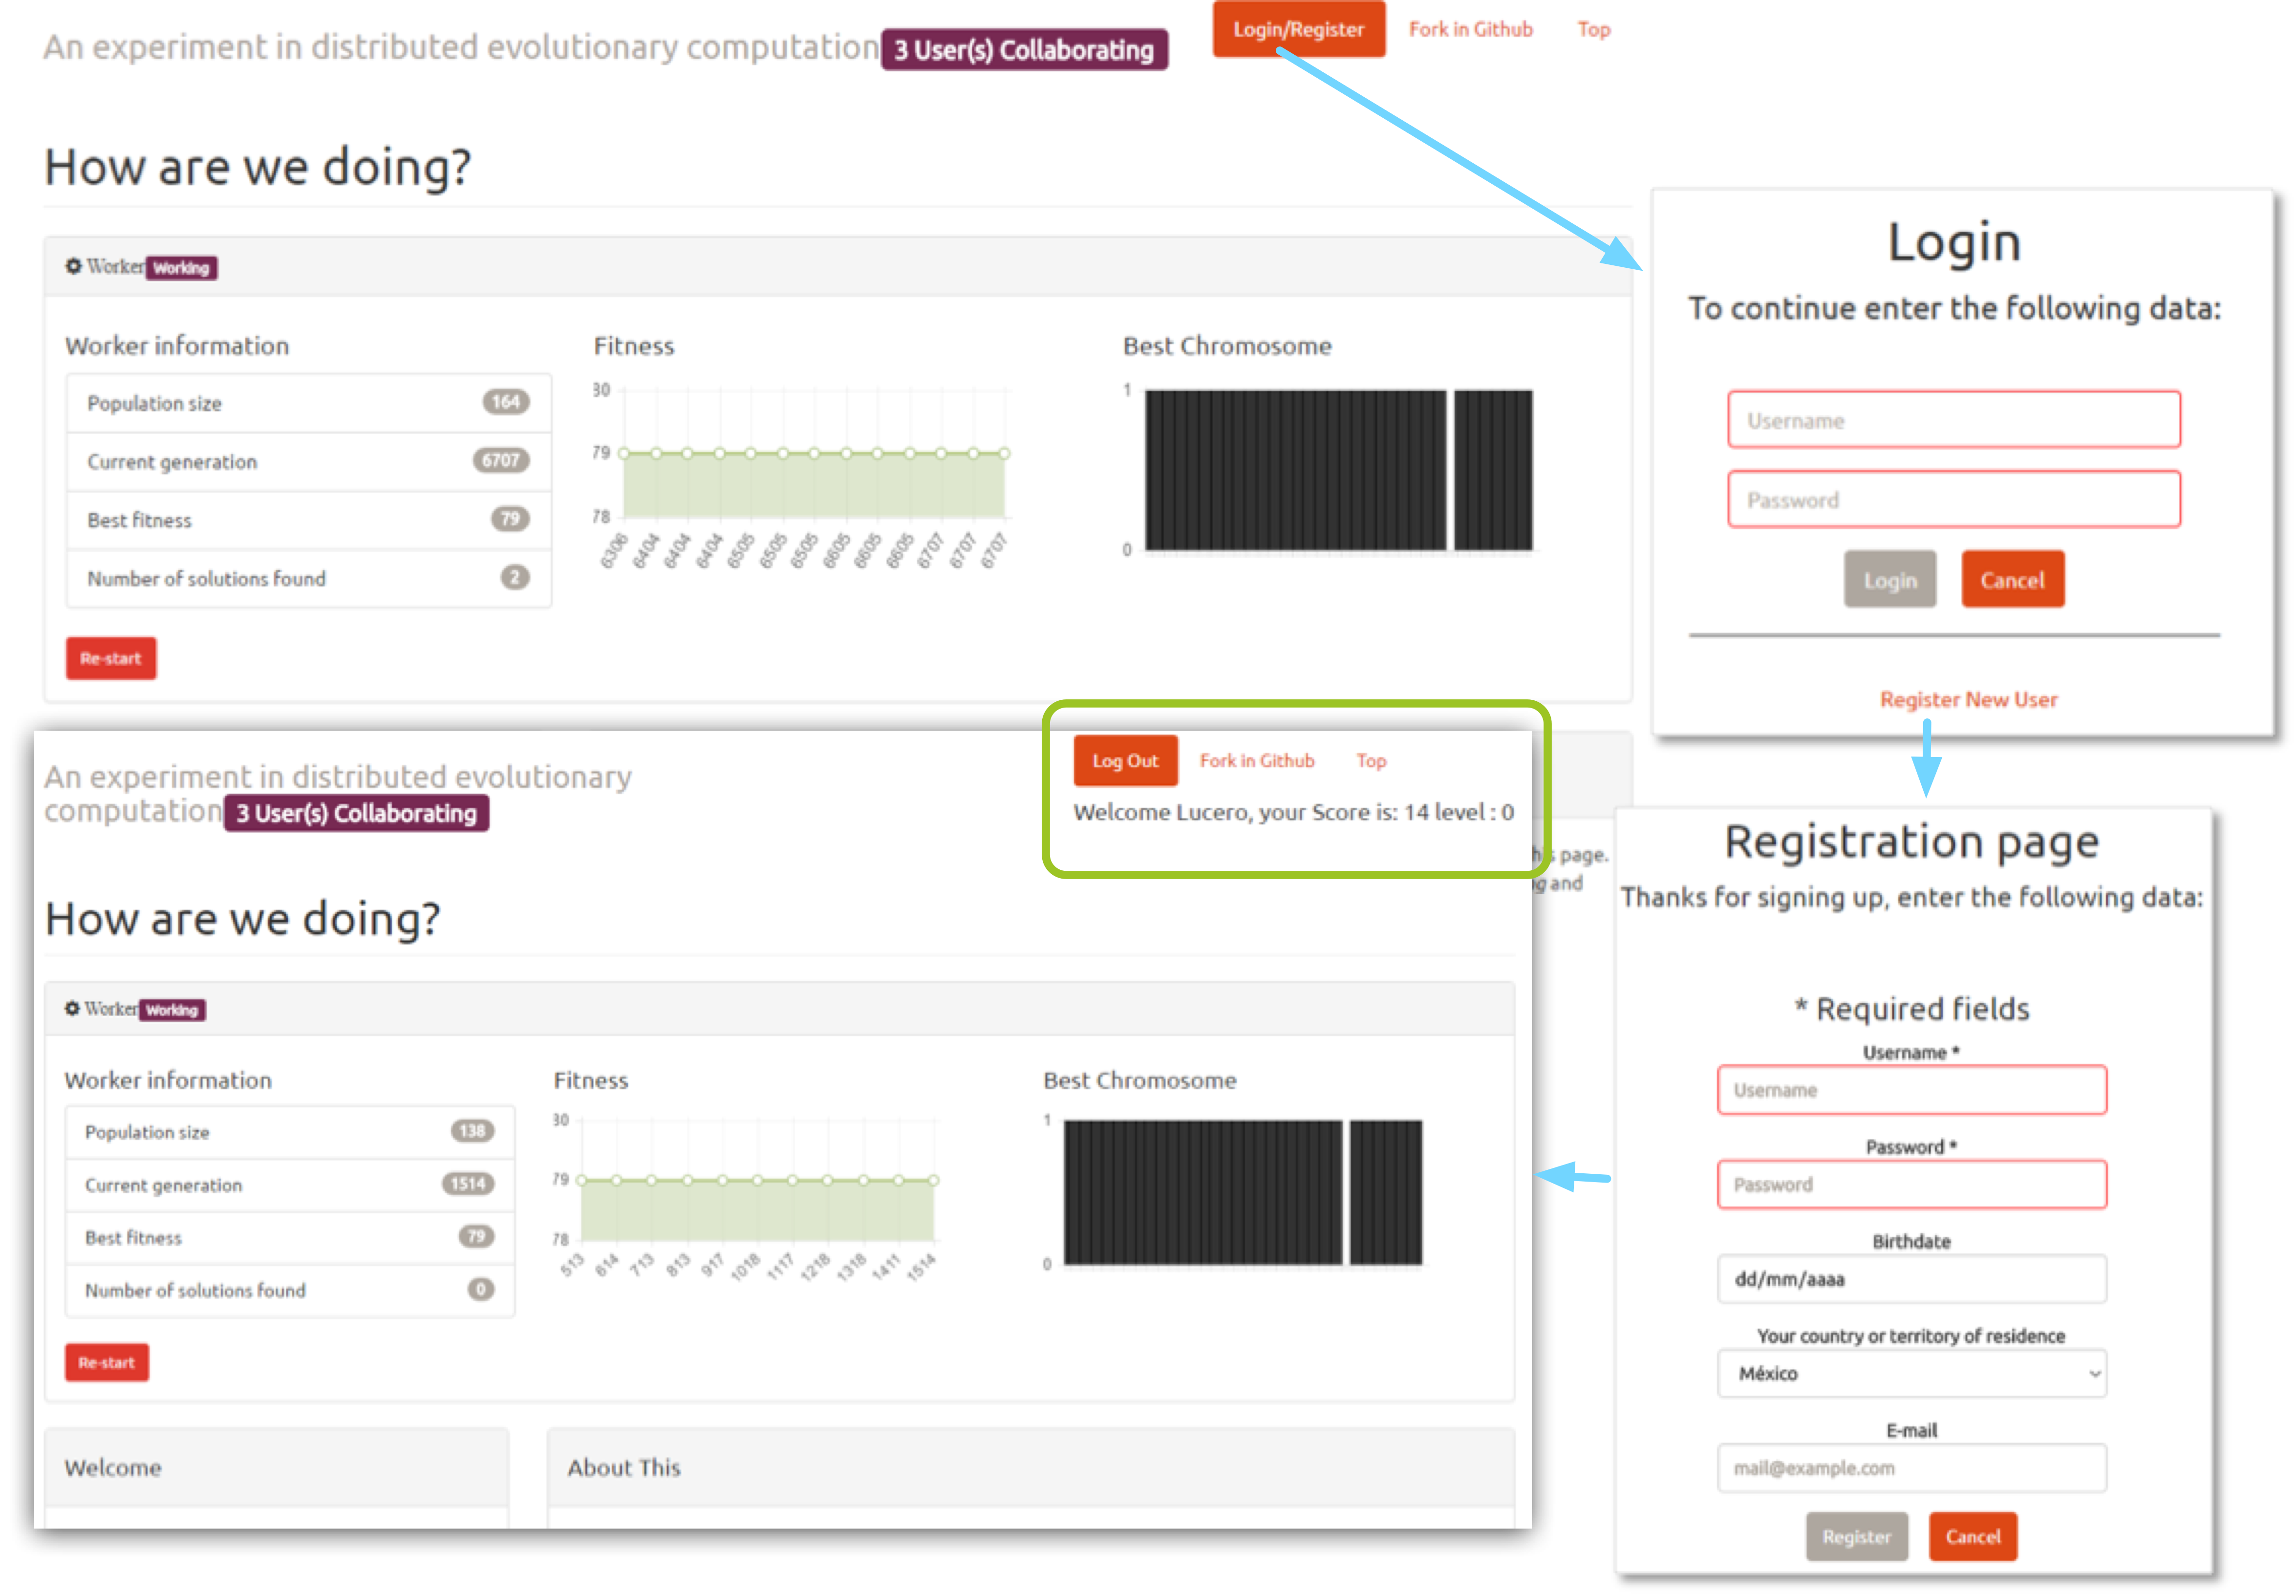
\includegraphics[width=5in]{img/login.png}
    \caption{ User interface: Landing page, and Login and registration dialogs.  
    }
    \label{fig:login}
\end{figure*}

\section{Experiment}
\label{sec:experiments}

In this experiment a gamification technique is applied to 
the {\sf NodIO} volunteer computing framework, using the 
particular version described in \cite{DBLP:conf/gecco/MereloCGCRV16,2016arXiv160101607M}.
The objective of the experiment is to test the kind of impact 
applying a gamification technique has on user engagement in this
particular application. In order to apply a rewarding system
user authentication had to be developed first. In earlier designs
this functionality was not desired because it was seen as a barrier 
for participation. After all the advantage of a browser based volunteer system
is precisely the minimum amount of user intervention needed to start.
The last thing a user wants to see is yet another registration form.
Then, the first design decision for this version is that registration is optional and simple as shown in Figure \ref{fig:login}. 

The gamification technique employed in this work is based on a rewarding mechanism  
\cite{dubois2013understanding}. In general rewards  consist of a reputation system 
with score points, levels and leader boards. Points are awarded to users in response of 
the accomplishment of certain activities that need to be encouraged. In these case
a point is awarded for each PUT sent to the server. Levels are a long
term achievement, in this case the level depends on the score:
\[ \text{level}(\text{score};a,b)= 
    \begin{cases} 
      0,                                    &  \text{score}\leq a\\    
      2(\frac{\text{score}-a}{b-a})^{2},    &  a\leq \text{score}\leq \frac{a+b}{2}\\
      1-2(\frac{\text{score}-b}{b-a})^{2},  & \frac{a+b}{2} \leq \text{score}\leq b\\
      1,                                    & \text{score}\geq b 
   \end{cases}
\]
The function returns a normalized value that is multiplied by the maximum level 
in this case 100. The variables $a$=100 and $b$=7360 are set to give users a rapid increase of 
levels at the beginning.
% \begin{figure*}[htbp]
%     \centering
%         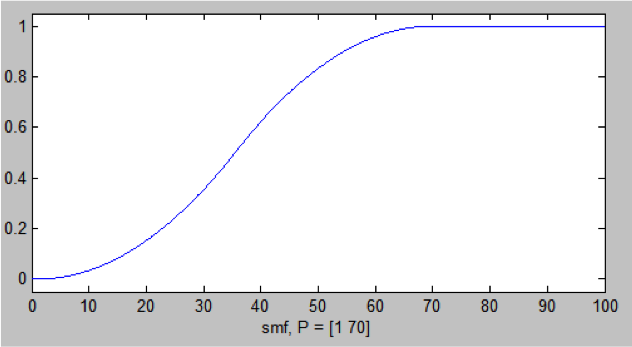
\includegraphics[width=2.5in]{img/s.png}
%     \caption{$S$ function used to assign the user's level.
%     }
%     \label{fig:s}
% \end{figure*}

After login, registered users are welcomed by their name, and they can see
their score and level. All users can see in a modal dialog the leader board.
While the modal is opened, the scores are refreshed every second. All other 
functionality is available to all users and is the same as the previous 
{\sf NodIO} version, showing the state of the current algorithm. 
In the front page a link to the open source code of the experiment was also 
available \url{https://github.com/lucero21/login-master} 


\subsection{Problem}
In the browser, each page visiting the experiment loads an WebWorker
that runs a local island of an evolutionary algorithm to solve a
multi-modal problem called {\em l-trap}, which has been used extensively 
as a benchmark for evolutionary algorithms \cite{fernandes2009using,nijssen2003analysis}. 
This function counts the number of bits in a sequence $l$ and assigns
the local maximum $a$ if it has got 0 bits and the global maximum $b$ if it has $l$
bits, this makes the  the fitness fall into a {\em trap} 
as the number of bits is increased, decreasing linearly until a change in slope 
is reached at point $z$, adding deceptive component for evolutionary algorithms. 
To increase the difficulty trap functions can be concatenated. 
In our case we have used $40$ concatenated traps. The trap function  defined as:   
\[ f(u)= 
    \begin{cases} 
      \frac{a}{z}(z-u) & \text{if } u\leq z\\
      \frac{b}{l-z} (u-z)& \text{otherwise} 
   \end{cases}
\]
% \begin{figure*}[htbp]
%     \centering
%         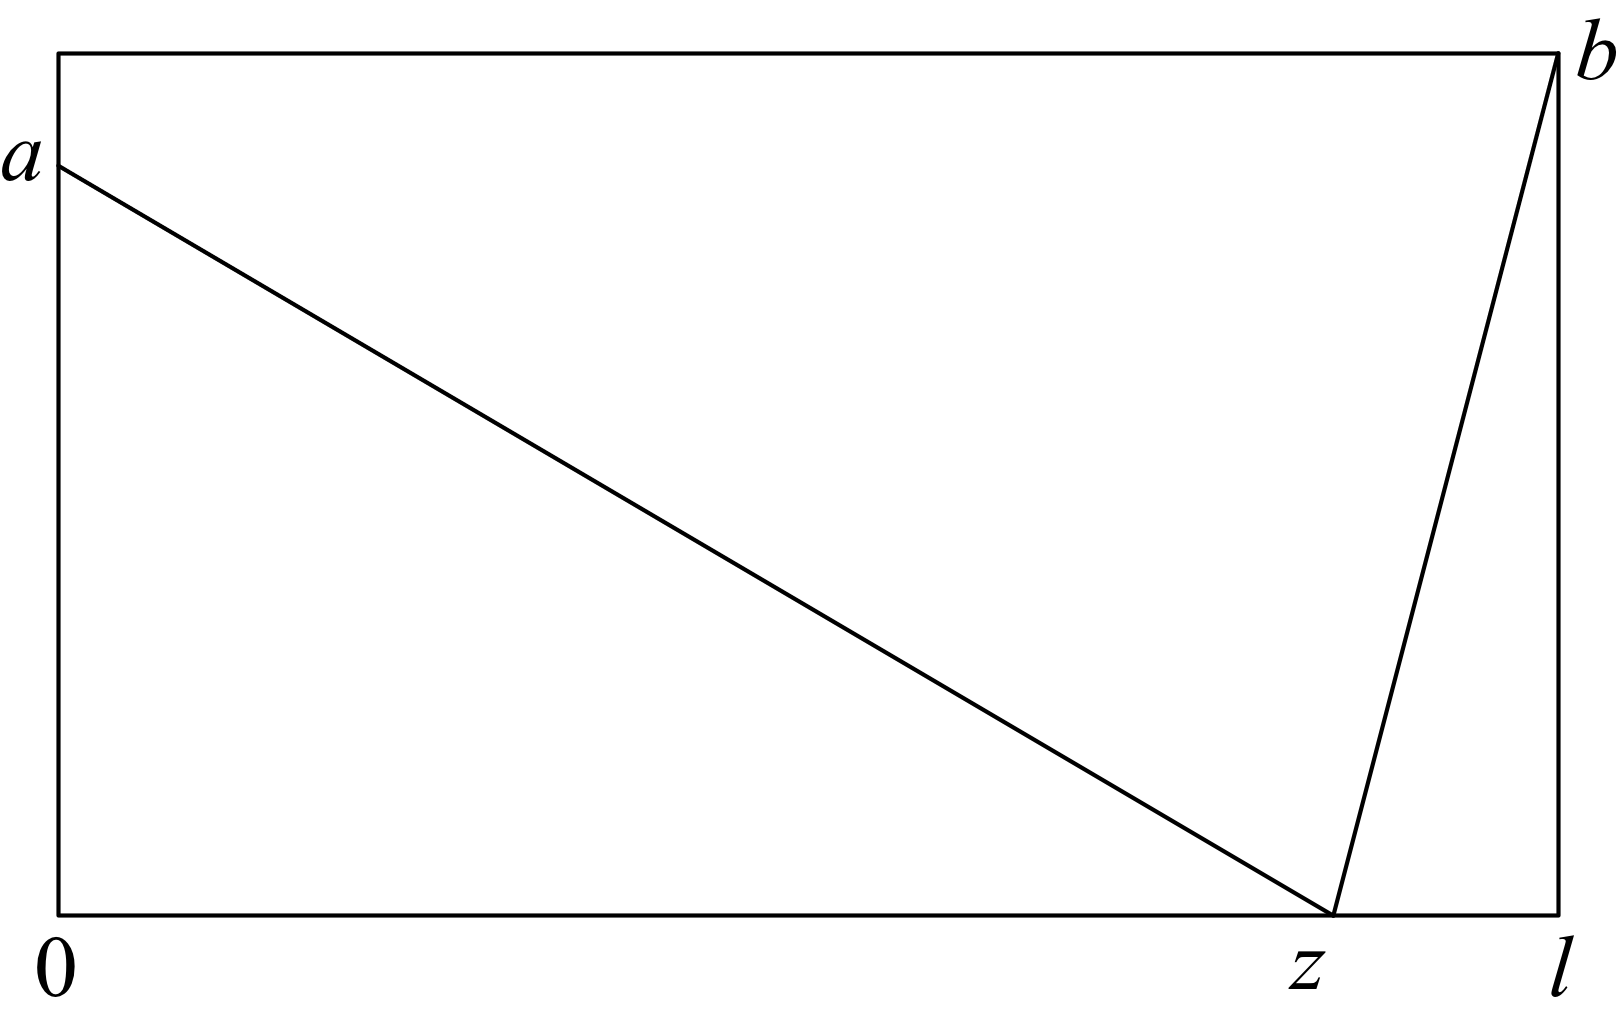
\includegraphics[width=2.5in]{img/trap.png}
%     \caption{Trap function.
%     }
%     \label{fig:trap}
% \end{figure*}
%

Each local GA had the following parameters, the initial population was randomly generated 
with sizes between 128 and 256 individuals, the period to send individuals to the server
was set at 100 local generations, the parameters for the trap function are $l$ = 4,
$a$=1, $b$ = 2, $z$=3 and a chromosome length of 160 bits.

We made a call to participation on November 23th, 
2016 through the authors' social networks: ``Asking again for your help, we are conducting a computational experiment
that requires computer power. Can we borrow some of your CPU? just visit the web page (link)
and leave the tab open. Be part of the TOP TEN, register so we can track your participation.
The experiment will run until November 27th, Thanks!.'' We also included links to register and a deadline. Users visiting the pageafter the dealine were presented with a thank you message and a static leader board. 
%

\subsection{Results}
\label{sec:results}

\begin{table}[h!tbp]
  \small
  \caption{ Log file record structure}
  \label{tab:record} 
  \centering
  \small
  \begin{tabular}{l  l}
    \hline\noalign{\smallskip}
    Attribute & Value \\
    \noalign{\smallskip}\hline\noalign{\smallskip}
    chromosome   & The individual sent to the server as a string of 160 bits.  \\ \hline
    fitness & fitness as an integer.  \\ \hline
    IP & IP address of the participant (later anonymized) .\\ \hline
    user & user-name or the string `anonymous'.  \\ \hline
    worker\_uuid & unique identifier of the HTTP Worker that sent the participation.   \\ \hline
    level &  level of user or the string `info' \\ \hline
    message & Only PUT messages were recorded in this experiment. \\ \hline
    timestamp & A time-stamp based on the Unix epoch\\ \hline
  \end{tabular}
\end{table}
%
At the end of the experiment the resulting log file (whose fields are shown in Table \ref{tab:record}) contained 933,513 contributions both 
registered users and anonymous volunteers. Registered users where responsible of around
90\% of the contributions. The JSON data recorded for each contribution is  presented 
in Table~\ref{tab:record}.  

\begin{figure}[h!tbp]
    \centering
        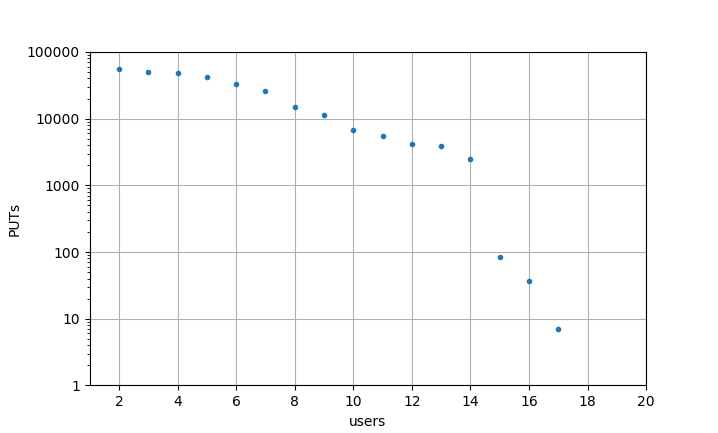
\includegraphics[width=2.3in]{img/puts_user.png}
        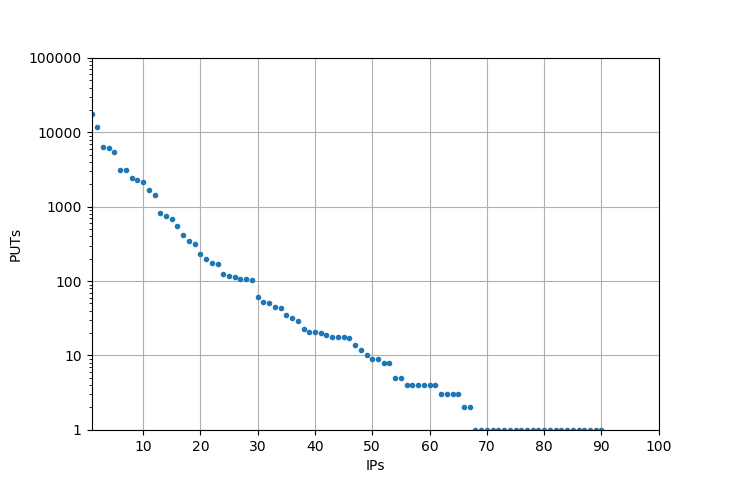
\includegraphics[width=2.3in]{img/puts_ip.png}
    \caption{Usage by registered (left) and anonymous (right) users.  Users are ranked by
        the number of requests sent, in the \emph{x} axis is the rank, and in the \emph{y} axis 
        number or PUTs in a logarithmic scale.}
    \label{fig:puts}
\end{figure}
%
Contributions are expressed as the number of HTTP PUT requests sent to the server, 
in Figure~\ref{fig:puts} a comparison between registered vs anonymous users is 
presented. There where only 18 registered users, and the exact number of anonymous
is not known as we only recorded the IP of the request, also a registered users 
could sometimes be anonymous too, this could be because the first time they visit
the application they automatically begin to work as anonymous. Nevertheless,
there were 91 distinct IPs that had `anonymous' as the user. In the plot of
anonymous users, some of the last in the rank could in fact be registered users, 
momentarily participating as anonymous. Even if this is not considered, only 
about 16\% of users attending the call decided to participate as named users. 
There is a notable difference in the amount of participation between the two
groups, and also in the slope of the plot.

%
\begin{figure*}[htbp]
    \centering
        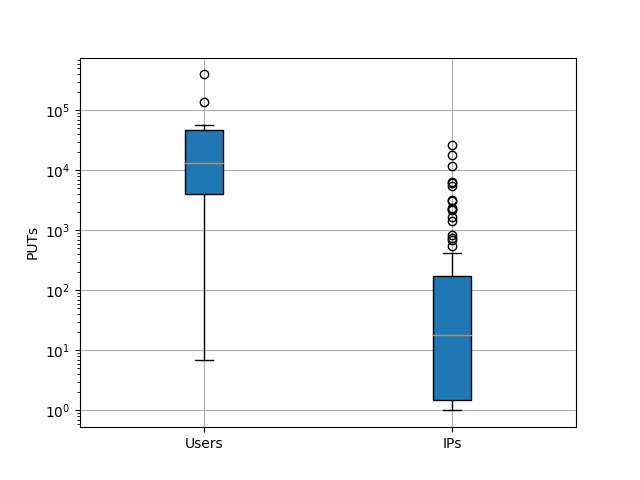
\includegraphics[width=4in]{img/puts_box.png}
    \caption{ Box-plot of the number of requests sent by registered users and anonymous IPs.
     In the \emph{y} axis are number or PUTs in a logarithmic scale.
    }
    \label{fig:box}
\end{figure*}
%
The box plot \ref{fig:box} of the amount of participation between the two groups, highlights
the difference and also the number of outliers in the groups. Two registered 
outliers where very important participants maybe competing between them. But
there where more outliers between anonymous IPs, and some of them could be related
to the same users. The lower quartile in in the users box-plot has more
spread, indicating a participation similar to the median of anonymous IPs.

%
\begin{figure*}[htbp]
    \centering
        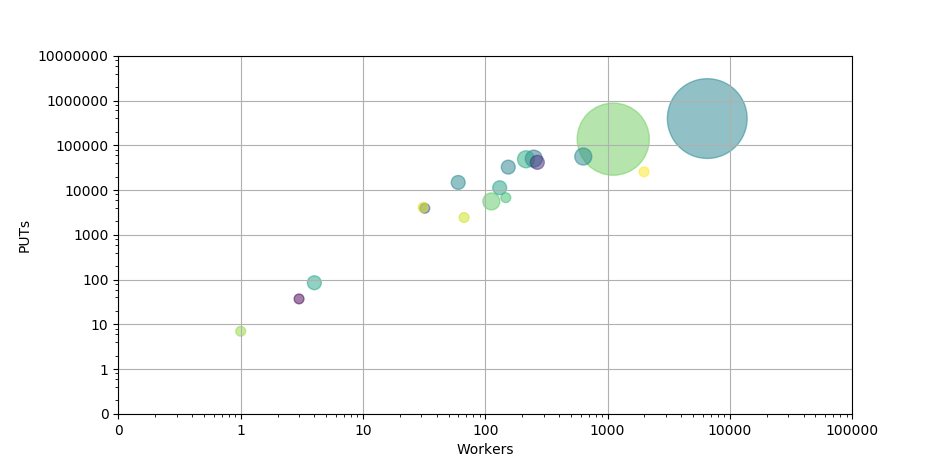
\includegraphics[width=5in]{img/workers_put_ip.png}
    \caption{ Participation of registered users. Each circle represents a user relating  
        in the \emph{x} axis the number of workers used and in the \emph{y} axis 
        number or PUTs in a logarithmic scale. The area of the circle is the number 
        of unique IPs used by the user.
    }
    \label{fig:worker-put-ips}
\end{figure*}
%
Figure~\ref{fig:worker-put-ips} gives an interesting view on the amount of
resources shared by registered users. The area of the circle is proportional
to the number of unique IPs used by each user, the user with more participation
used a total of 66 different IPs, this number could be related with the number
of devices used during the participation. There are some users that using less
devices participated more, this could mean a more powerful device, faster 
Internet connection or simply more time spent participating.

User engagement is related to the amount of time a user spends in the 
application. Figure~\ref{fig:puts-time} shows to important aspects of
engagement, the overall time spent and the amount of resources shared
in that time. Registered users where more engaged during the experiment.
They contribute more resources during longer periods of time.

%
\begin{figure*}[htbp]
    \centering
        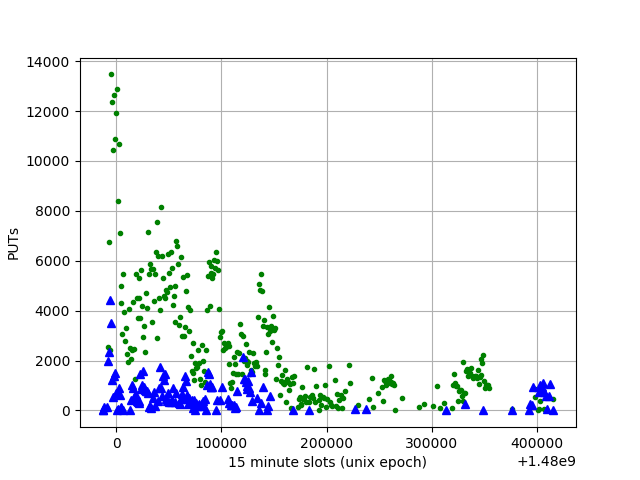
\includegraphics[width=4in]{img/puts_by_time.png}
    \caption{Number of PUTs by User or IP in 15 minute slots.
    }
    \label{fig:puts-time}
\end{figure*}
%
\begin{figure*}[htbp]
    \centering
        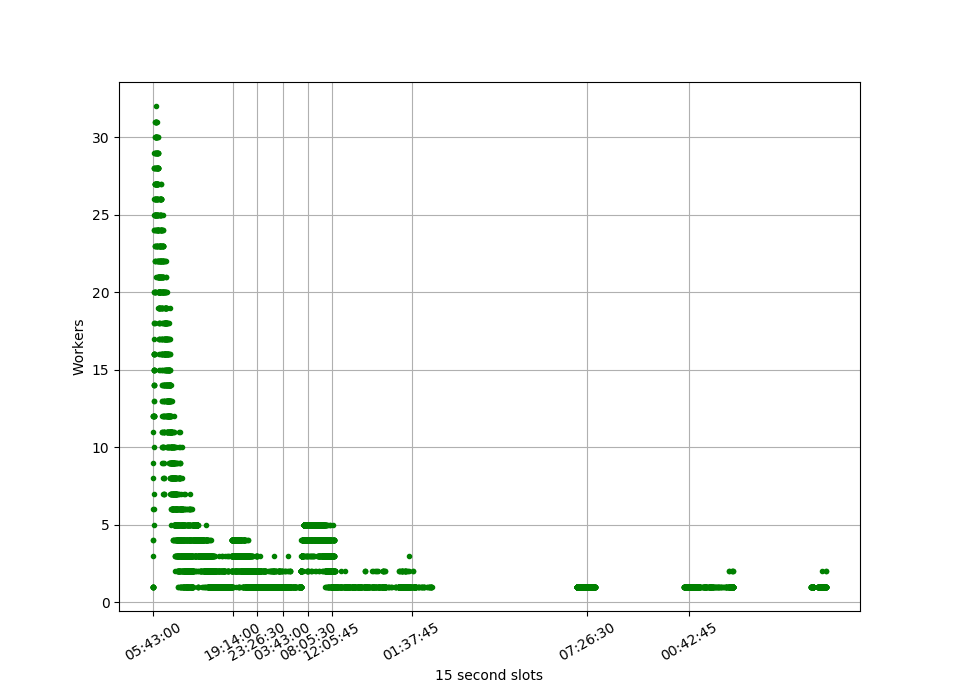
\includegraphics[width=5in]{img/workers_best_user.png}
    \caption{ Number of workers used by the top ranked user in 15 minute slots.
    }
    \label{fig:top-user}
\end{figure*}
%
The participation of the top ranked user is presented in 15 seconds time slots in
Figure~\ref{fig:top-user}. In the beginning this user was using more than 30
workers, this means that more than 30 tabs of the page where open at the
same time, perhaps using several computing devices. Some users reported that 
they wanted to test the limits of their own systems, checking the percentage of
CPU they where using. 


\section*{Acknowledgments}

This work has been supported in part by: Ministerio espa\~{n}ol de
Econom\'{\i}a y Competitividad under project TIN2014-56494-C4-3-P
(UGR-EPHEMECH).

\bibliographystyle{splncs03}

\bibliography{../../bib/biblio,../../bib/evospace-i,../../bib/volunteer,../../bib/geneura}

\end{document}
